\documentclass[dissertation.tex]{subfiles}
\begin{document}

\chapter{Automatic composition}

This chapter describes a generative probabilistic sequence model for automatic
composition of polyphonic music. We introduce a local representation for
polyphonic scores as well as the preprocessing steps performed to construct
the corpus of Bach chorales used throughout the remainder of our work. In addition,
we describe the architecture, design decisions, and techniques used to construct
and train our model.

\section{Constructing a corpus of encoded scores}

We restrict the scope of our investigation to Bach chorales for the following reasons:
\begin{enumerate}
  \item The Baroque style employed in Bach chorales has specific guidelines
    \cite{piston1978harmony} (i.e.\ no parallel fifths) and stylistic elements
    (i.e. voice leading) which can be use to qualitatively evaluate success
  \item The structure of chorales are regular: all chorales have four parts and
    consist of a melody in the Soprano part harmonized by the Alto, Tenor, and
    Bass parts. Additionally, each chorale consists of a series of \emph{phrases}:
    groupings of consecutive notes into a unit that has complete musical sense
    of its own\cite{nattiez1990music}. It is well known\todo{cite} that Bach
    denoted ends of phrases with fermatas\todo{refer back to background}.
  \item The Bach chorales have become a standardized corpus routinely studied
    by aspiring music theorists\cite{white2002guidelines}
\end{enumerate}
The Bach chorales, indexed by the Bach-Werke-Verzeichnis (BWV) numbering
system\cite{butt1999bach}, are conveniently provided by
\texttt{music21}\cite{Scott2015}.

\subsection{Preprocessing}

Motivated by the transposition invariance of music and prior practice
\cite{mozer1994neural} \cite{Eck2002} \cite{franklin2004recurrent}
\cite{franklin2005jazz}, the keys of each score was first analyzed using the
Krumhansl Schmuckler key-finding algorithm \cite{krumhansl2001cognitive} and
then transposed according to \todo{Table XYZ} such that the transposed key is
C-major for major mode scores and A-minor for minor mode scores.

Next, scores are quantized. Our model uses a quantization of one $1/16$th note
per frame, exceeding the time resoltuions of \cite{Boulanger-Lewandowski2012}
\cite{Eck2002} by 2x, \cite{hild1991harmonet} by 4x, and
\cite{bellgard1994harmonizing} by 8x.

\todo{All dynamics information is removed.}
We consider only note pitches and durations, neglecting changes in timing
(e.g. ritardandos), dynamics (e.g. crescendos), and stylistic notations (e.g.
accents, staccatos, legatos).

An example of the effects of our preprocessing steps is provided in
\autoref{fig:score-effects-preproc} (sheet music notation) and
\autoref{fig:piano-roll-effects-preproc} (piano roll) \todo{Reference
background}.

\begin{figure}[htbp]
    \centering
    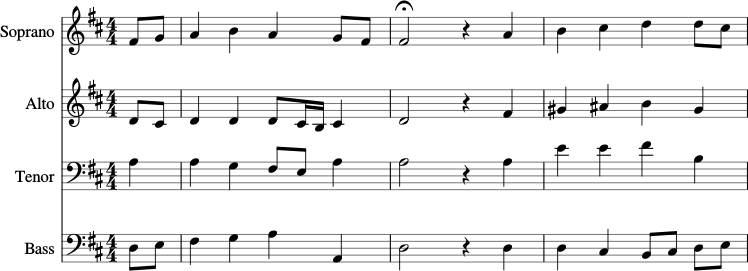
\includegraphics[width=0.8\linewidth]{Figures/bwv133-6-original-score-1.png}
    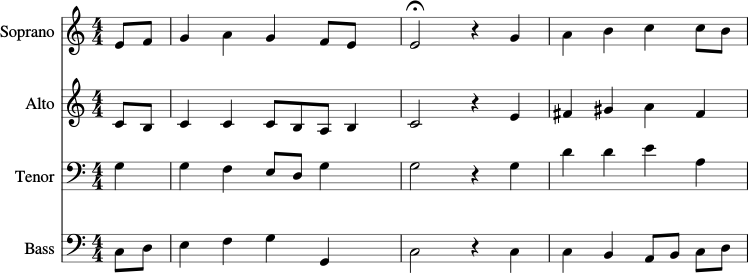
\includegraphics[width=0.8\linewidth]{Figures/bwv133-6-preproc-score-1.png}
    \caption{First 4 bars of JCB Chorale BWV 133.6 before (top) and after (bottom) preprocessing. Note
    the transposition down by a semitone to C-major as well as quantization of the
    semiquavers to quavers in Alto bar 2.}
    \label{fig:score-effects-preproc}
\end{figure}

\begin{figure}[htpb]
    \centering
        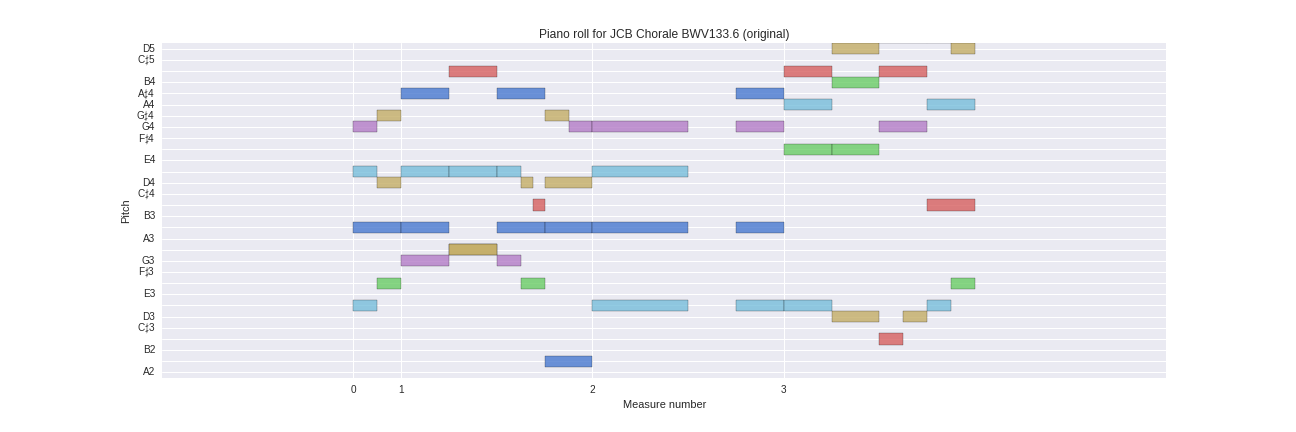
\includegraphics[width=1.0\linewidth]{Figures/bwv133-6-original-piano-roll.png}
        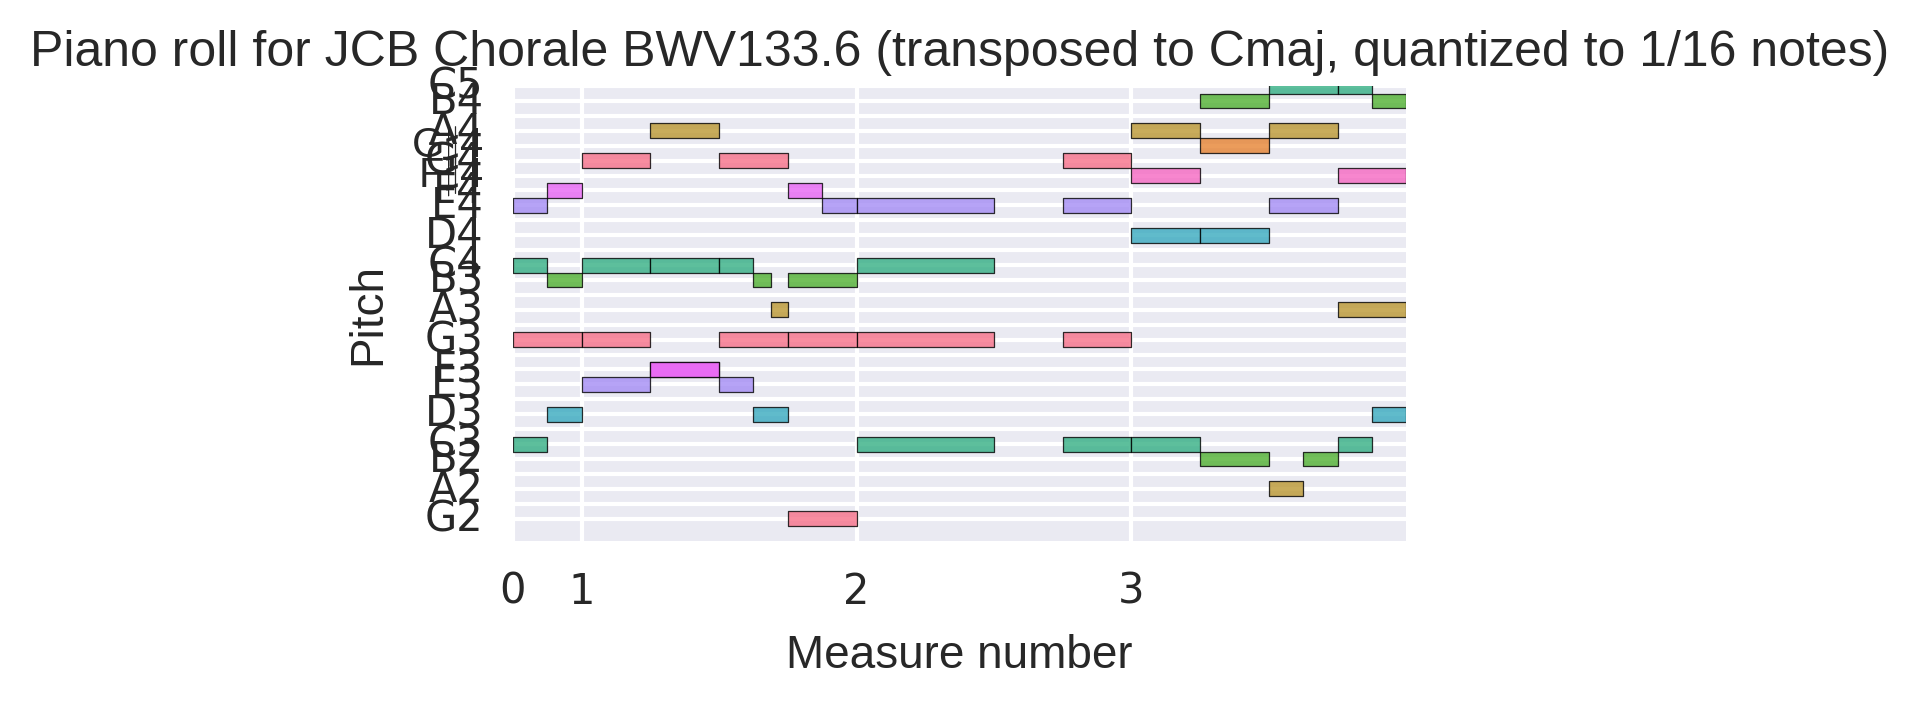
\includegraphics[width=1.0\linewidth]{Figures/bwv133-6-preproc-piano-roll.png}
    \caption{Piano roll representation of the same 4 bars from \autoref{fig:score-effects-preproc}
    before and after preprocessing.}
    \label{fig:piano-roll-effects-preproc}
\end{figure}


\subsection{Sequential encoding of musical data}

Similar to \cite{todd1989connectionist}, we represent polyphonic scores using a
localist frame-based representation where time is discretized into constant
timestep \emph{frames}. Frame based processing forces the network to learn the
relative duration of notes, a counting and timing task which
\cite{gers2002learning} demonstred LSTM is capable of. Consecutive frames are
separated by a unique delimiter (``$|||$''' in \todo{Figure of score encoded in
text}).

Each frame consists of a sequence of $\langle \text{Note}, \text{Tie} \rangle$
tuples where $\text{Note} \in \{0,1,\cdots,127\}$ represents the MIDI pitch of
a note and $\text{Tie} \in \{T,F\}$ distinguishes whether a note is tied with a
note at the same pitch from the previous frame or is articulated at the current
timestep. \todo{Order of SATB parts, bass rooting}.

The above specification describes our initial encoding. Later in our work
\todo{reference}, we found that this encoding resulted in unrealistically long
phrase lengths. Including fermatas (represented by ``(.)'' in \todo{Figure of
encoded score}, which Bach used to denote ends of phrases, solves this problem.

Finally, for each score a unique start symbol %(``ї'' in \todo{Figure})
and end symbol %(``ћ'' in \todo{Figure})
are appended to the beginning and end
repsectively. This causes the model to learn to initialize itself when given
the start symbol and allows us to determine when a composition generated by
the model has concluded.

Observe that our encoding is sparse: unarticulated notes are not encoded. It is
also variable length as anywhere from zero to four (in the case of chorales,
more for arbitrary polyphonic scores) notes. Finally, the explicit
representation of tied notes vs articulated notes solves the problem plaguing
\cite{Eck2002}\cite{eck2008learning} \cite{Liu2014} \cite{Brien2016} where
multiple articulations at the same pitch are indistinguishable from a single
note with the same duration.

Additionally, notice that our encoding avoids hand-engineered features such as
pitch representations which are psychochologically-based \cite{mozer1994neural}
or harmonically-based \cite{franklin2004recurrent}
\cite{laden1989representation}. This is intentional and is motivated by
numerous reports \cite{bengio2009learning}\cite{Bengio2011} suggesting that
that a key ingredient in deep learning's success is its ability to learn good
features from raw data.





\begin{figure}[htpb]
    \centering
    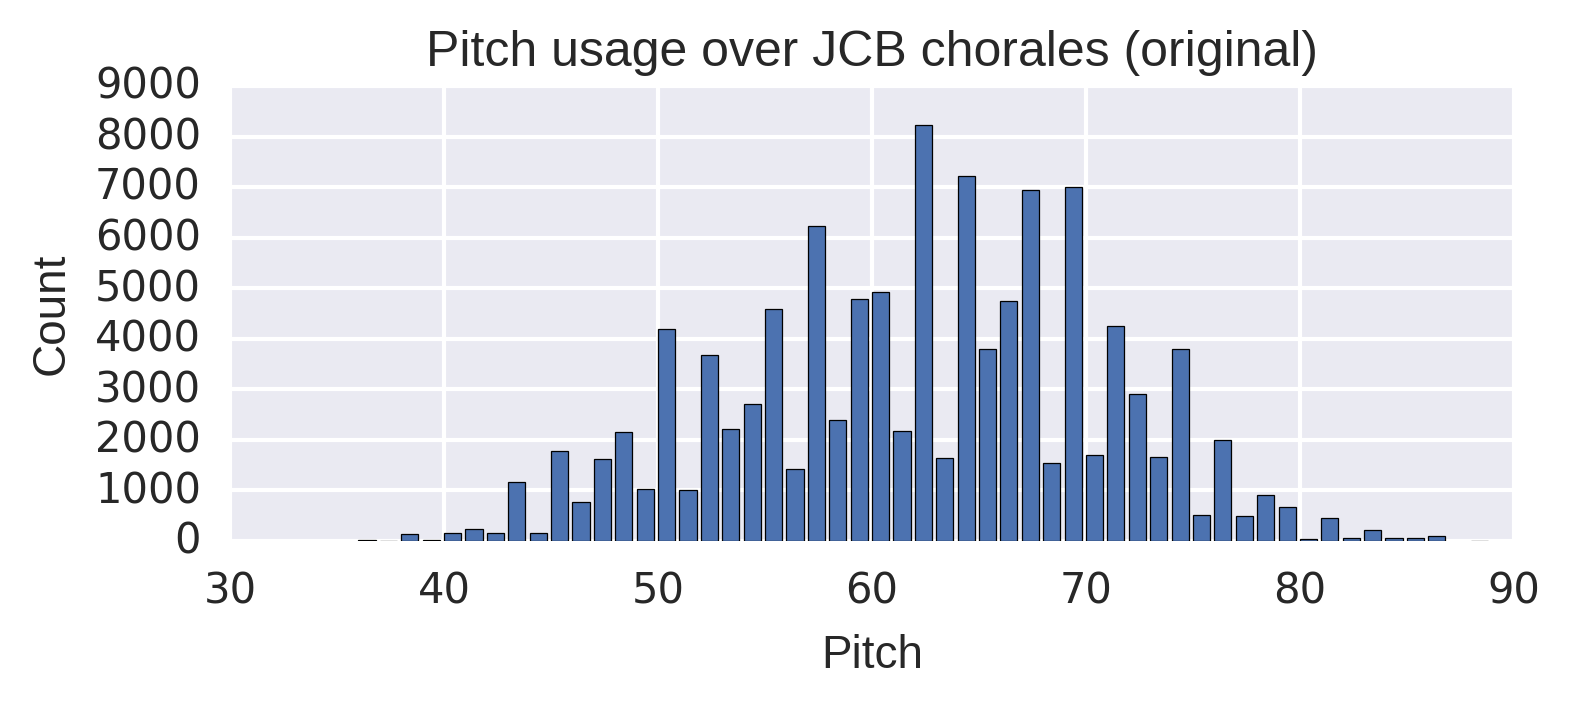
\includegraphics[width=1.0\linewidth]{Figures/pitch-usage-original.png}
    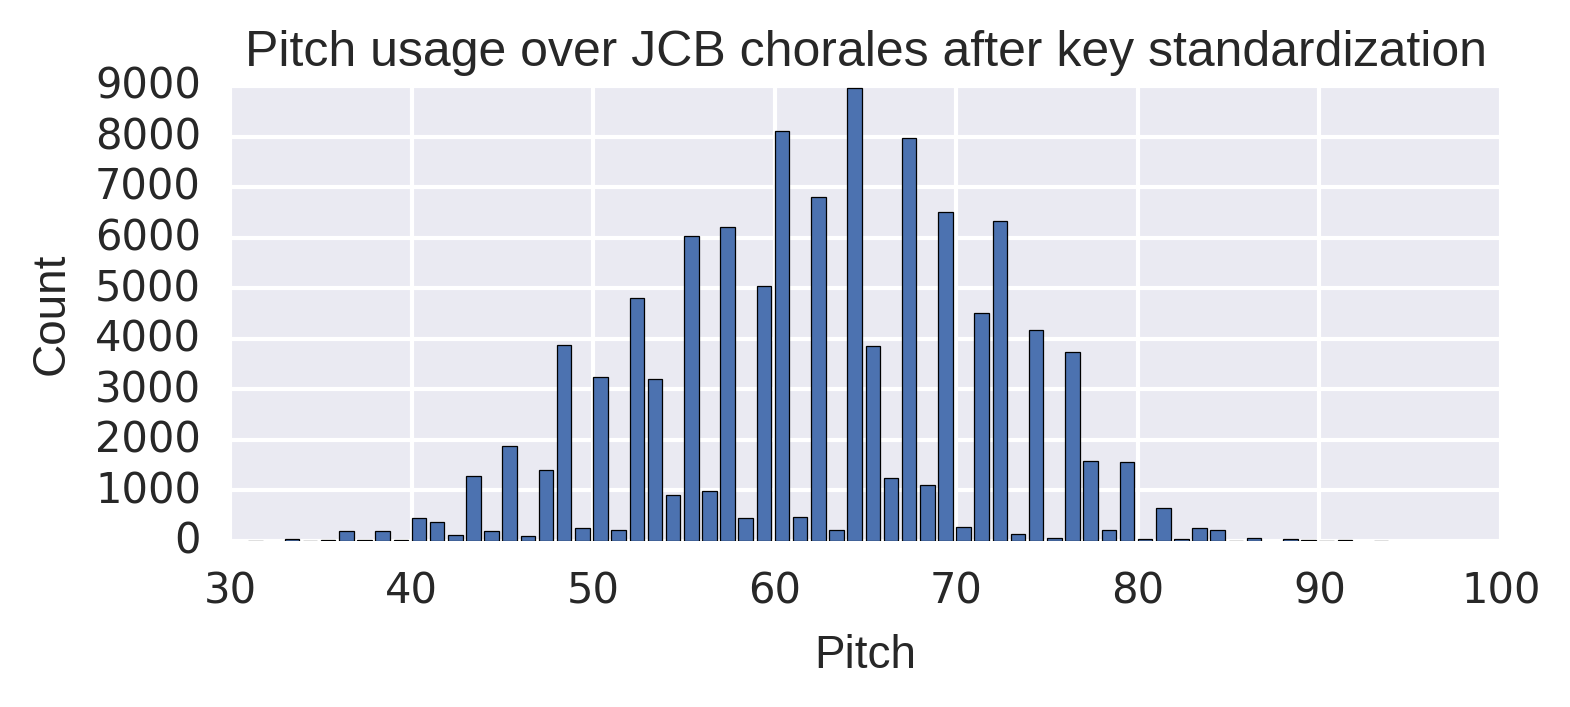
\includegraphics[width=1.0\linewidth]{Figures/pitch-usage-preproc.png}
    \caption{Pitches before and after key standardization}
    \label{fig:pitch-key-standardization}
\end{figure}

\begin{figure}
    \centering
    \begin{subfigure}[b]{0.48\textwidth}
        \centering
        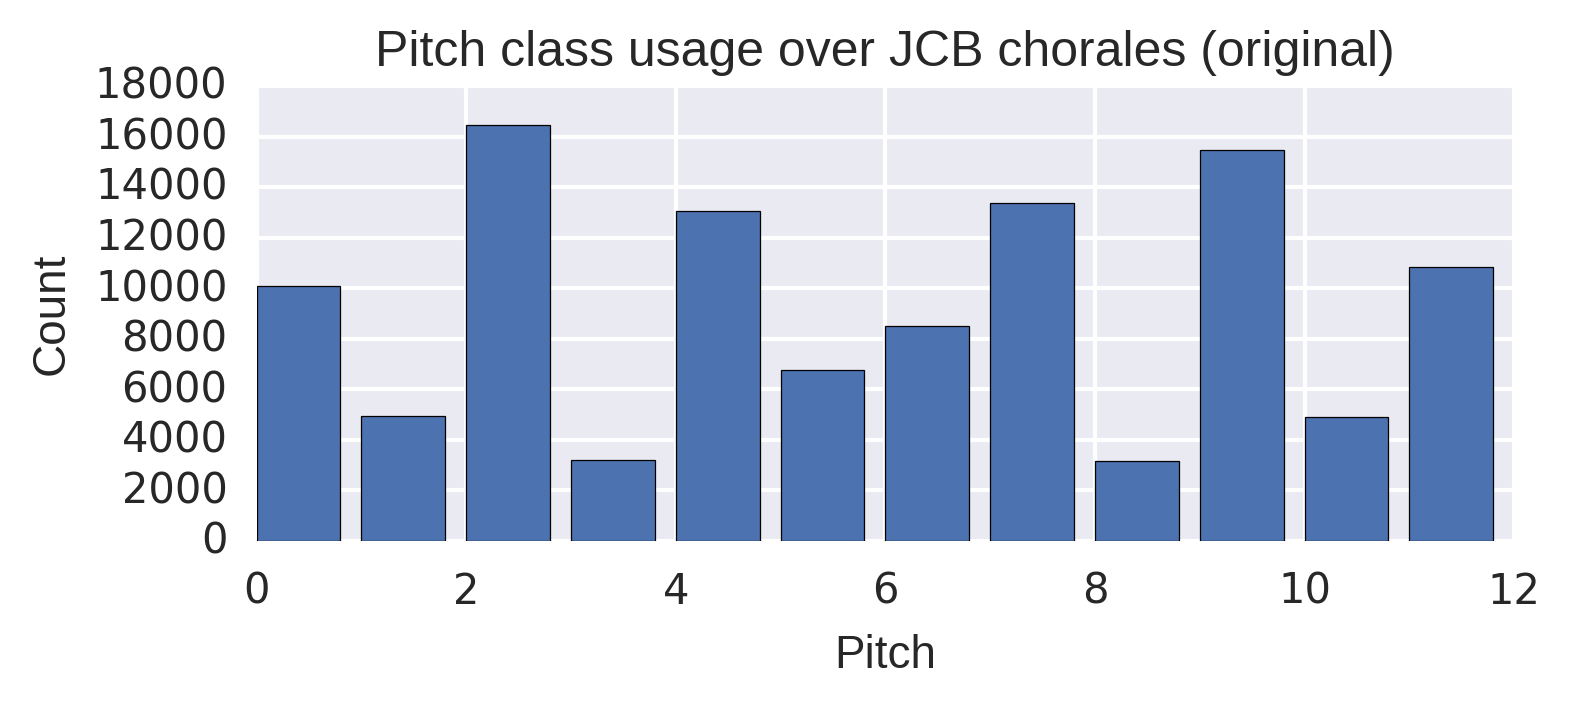
\includegraphics[width=1.0\linewidth]{Figures/pitch-class-usage-original.png}
    \end{subfigure}
    \begin{subfigure}[b]{0.48\textwidth}
        \centering
        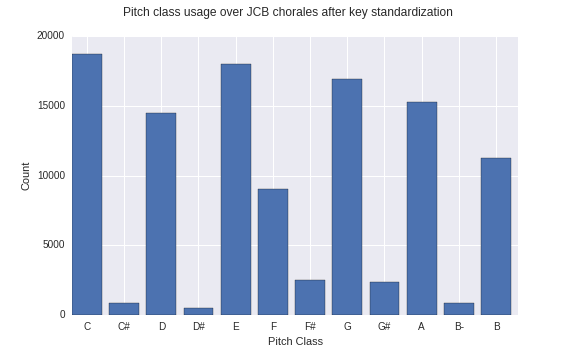
\includegraphics[width=1.0\linewidth]{Figures/pitch-class-usage-preproc.png}
    \end{subfigure}
    \caption{Pitch classes before and after key standardization}
    \label{fig:pc-key-standardization}
\end{figure}

\begin{figure}[htpb]
    \centering
    \begin{subfigure}[t]{0.48\textwidth}
        \centering
        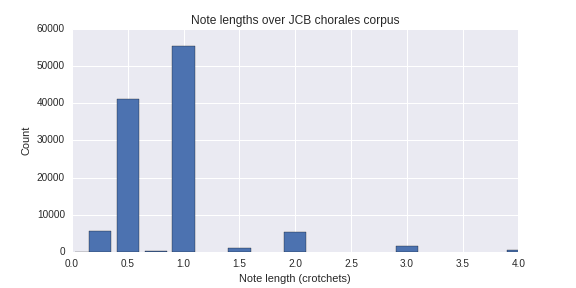
\includegraphics[width=1.0\linewidth]{Figures/note-lengths-original.png}
    \end{subfigure}
    ~
    \begin{subfigure}[t]{0.48\textwidth}
        \centering
        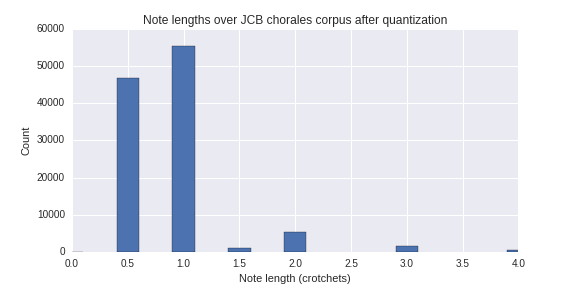
\includegraphics[width=1.0\linewidth]{Figures/note-lengths-quantized.png}
    \end{subfigure}
    \caption{Effects of time quantization on note durations}
    \label{fig:note-lengths-time-quantization}
\end{figure}

\begin{figure}[htpb]
    \centering
    \begin{subfigure}[t]{0.48\textwidth}
        \centering
        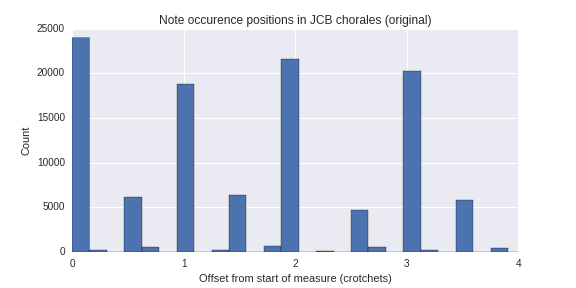
\includegraphics[width=1.0\linewidth]{Figures/meter-usage-original.png}
    \end{subfigure}
    ~
    \begin{subfigure}[t]{0.48\textwidth}
        \centering
        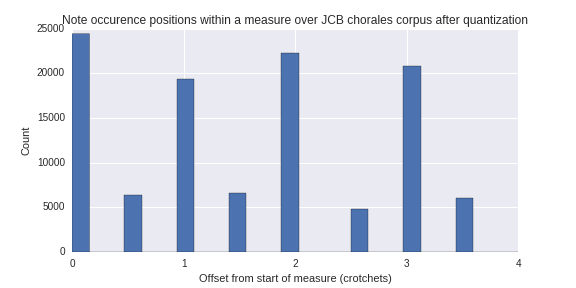
\includegraphics[width=1.0\linewidth]{Figures/meter-usage-quantized.png}
    \end{subfigure}
    \caption{Effects of time quantization on meter}
    \label{fig:meter-time-quantization}
\end{figure}



\section{Model description}

Unlike many prior models for music data, we avoid injection of
domain-specific knowledge into our models such as distinguishing between chords
versus notes \cite{hild1991harmonet}\cite{mozer1994neural} \cite{Eck2002} and
explicitly modelling of meter \cite{eck2008learning} or motifs
\cite{feulner1994melot}.

\subsubsection{Sequential processing and sampling}

Following \cite{1994neural}, we will train the model to predict a probability
distribution over all possible tokens at time $t+1$ using the token at time
$t$. We also employ \emph{teacher forcing}\cite{williams1989learning}, where
the target outputs instead of the actual outputs (i.e. most likely predicted
tokens for time $t+1$) as recurrent inputs since the model predictions may not
yet be correct during the early iterations of training.

We will train our RNNs to predict a distribution for the next character
$\x_{t+1}$ after the RNN has processed the sequence $\x_{1:t}$,
yielding a model which factorizes the sequence probability
\begin{equation}
    P(\x_{1:T}) = \prod_{t=1}^T P(\x_t | \x_{1:t-1} )
\end{equation}
Modeling this probability distribution over sequences is analogous to the
\textbf{language modeling} from speech recognition.

Note that the factorization of conditional distributions \emph{assumes a
sequential ordering in $t$}. This property is desirable as it enables sampling
from the model to generate new transcriptions by sampling from $P(\x_t |
\x_{1:t-1})$ at each timestep $t$ and using the sampled value as the next
input.

\subsection{Parameter estimation of recursive neural networks}


\subsubsection{Modeling probabilities using the Boltzmann distribution and cross-entropy error criterion}

The parameters to the model are estimated in order to minimize the error
between the network outputs and provided labels. For language modeling, the
outputs $\y_t$ should parameterize a distribution for the next character
$P(\x_{t+1} | \x_{1:t})$. Suppose each input has finite support (i.e.
$\x_t \in [1,2,\cdots,K]$). If we choose the outputs to be $K$ dimensional
(i.e. $\y_t \in \RR^K$) then the \textbf{Boltzmann distribution}
(\autoref{eq:boltzmann-dist}) can be used:

\begin{equation}
    \label{eq:boltzmann-dist}
    P(\x_{t+1} = s | \x_{1:t})
    = \frac{\exp \left(-\y_{t,s}/T\right) }{ \sum_{k=1}^{K} \left(\exp -\y_{t,k}/T\right)}
\end{equation}

$T \in \RR^+$ is a \textbf{temperature} parameter \todo{relate to sampling}.

The labels provided are the actual next characters $\x_{t+1}$. Viewing
such labels as discrete probability distributions will all mass on a single atom,
one measure of difference between predictions and \todo{justify cross-entropy}

\section{Polyphonic modeling}

\cite{Nayebi2015} reports LSTMs significantly
outperform GRUs in music applications.

\section{Technical details}

\todo{We use teacher forcing \cite{williams1989learning}}

We construct multi-layer LSTM models with \texttt{num\_layers} number of
layers, each containing \texttt{rnn\_size} hidden units. The inputs $x_t$ are
one-hot-encoded before being passed through a \texttt{wordvec}-dimensional
vector-space embedding layer, which compresses the dimensionality down from
$|V| \approx 140$ to $\texttt{wordvec}$ dimensions. Dropout layers were added
between LSTM connections in both depth and time dimensions all with dropout
probability $\texttt{dropout} \in [0,1]$.

We build our models using the \texttt{torch7} framework and
an optimized implementation of LSTMs provided by \texttt{torch-rnn} \todo{cite}.

Models were trained using RMSProp \todo{cite} with batch normalization \todo{cite}
and an initial learning rate of $2 \times 10^{-3}$ decayed by $0.5$ every $5$
epochs. The back-propogation through time gradients were clipped
at $t$ \todo{cite Mikolov} and truncated after \texttt{seq\_length} time steps.
We use a mini-batch size of $50$.

\subsection{Multi-GPU implementation}

To accelerate model training, we parallelize models across multiple GPUs. This is possible
thanks to the summation operation in noisy gradient estimators:

\begin{equation}
  \frac{1}{N} \sum_{i=1}^N \nabla L_i(\theta) \approx \frac{1}{N} \sum_{i=1}^N \nabla L_i(\theta)
\end{equation}
\todo{Real citations on noisy gradient}

In particular, training RNNs with hidden state requires sequential traversal
of the dataset. Parallelizing sequential iteration is accomplished by first segmenting
into equal length segments and then initializing parallel iterators each
pointing at a different segment. Each iterator sequentially reads data
into GPU memory.

Model parameters are broadcast out to all GPUs on each \texttt{forward} pass
and gradients are accumulated during each \texttt{backward} pass.

Research in grid LSTMs suggests that we can go deeper by introducing
gates along the depth dimension to help permit information flow \todo{cite gird LSTMs}.

\section{Results}

Compare with \cite{Allan2005} and \cite{Brien2016}.

\printbibliography

\end{document}
